\chapter{Opis interfejsu użytkownika}

\section*{Panel logowania}

Jak pokazano na Rys. \ref{fig:login_panel}, panel logowania umożliwia autoryzację użytkownika przed uzyskaniem dostępu do głównego interfejsu systemu. Formularz składa się z dwóch pól: \texttt{Login} oraz \texttt{Password}, oraz przycisku \textbf{Zaloguj}.

W przypadku poprawnych danych, użytkownik zostaje przekierowany do głównego panelu systemu. Jeśli jednak dane logowania są nieprawidłowe, system wyświetla stosowny komunikat błędu za pomocą okna typu \texttt{JOptionPane}. Panel zapewnia podstawową walidację pustych pól i poprawności danych logowania.

\begin{figure}[H]
\centering
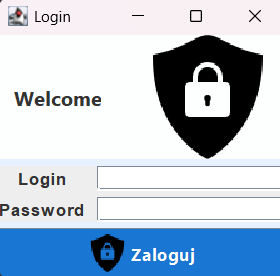
\includegraphics[width=0.4\textwidth]{figures/workApl/login_panel.png}
\caption{Panel logowania do systemu}
\label{fig:login_panel}
\end{figure}

\clearpage

\section*{Główny panel sekretariatu}

Na Rys. \ref{fig:mainpanel} widoczny jest główny panel sekretariatu. Panel ten jest centralnym miejscem zarządzania danymi w systemie. Wyświetla on tabelę ze wszystkimi zajęciami zapisanymi w bazie danych.

Użytkownik ma do dyspozycji przyciski:
\begin{itemize}
    \item \textbf{Dodaj} – otwiera formularz umożliwiający dodanie nowych zajęć,
    \item \textbf{Edytuj} – pozwala zmodyfikować zaznaczony rekord,
    \item \textbf{Usuń} – usuwa wybrane zajęcia z bazy,
    \item \textbf{Zastosuj filtry} – uruchamia filtrację danych,
    \item \textbf{Odśwież} – ładuje wszystkie dane ponownie.
\end{itemize}

Filtrowanie zajęć możliwe jest przez rozwijane listy, w których użytkownik może wybrać: salę, grupę lub typ zajęć. Dane prezentowane są w tabeli \texttt{JTable}, umieszczonej w kontenerze \texttt{JScrollPane}.

\begin{figure}[H]
\centering
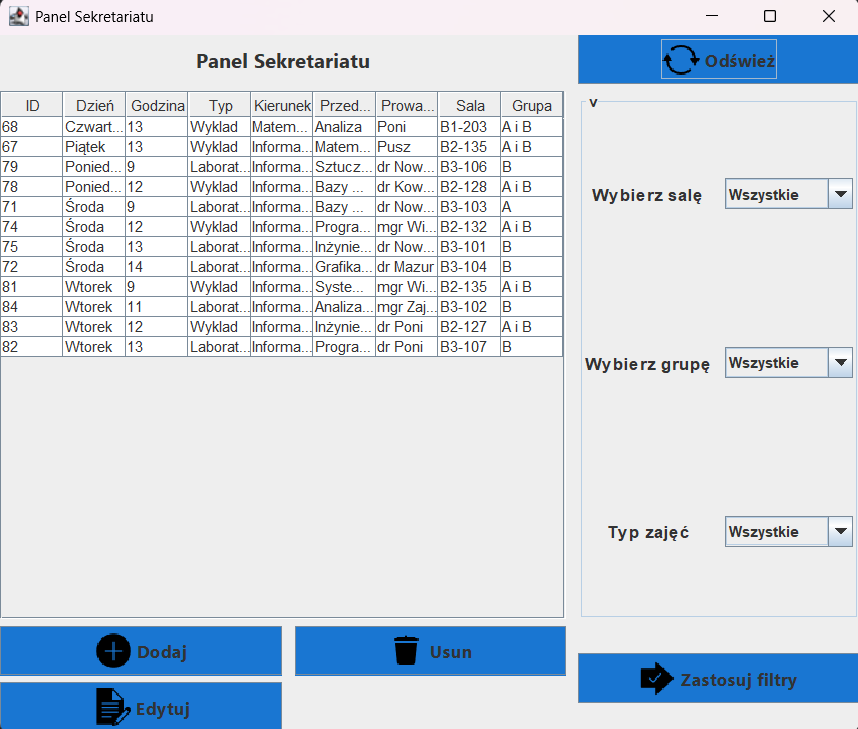
\includegraphics[width=0.9\textwidth]{figures/workApl/mainpanel.png}
\caption{Główny panel sekretariatu z listą zajęć i filtrowaniem}
\label{fig:mainpanel}
\end{figure}

\clearpage

\section*{Formularz dodawania zajęć typu Wykład}

Rysunek \ref{fig:add_wyklad} przedstawia panel umożliwiający dodawanie zajęć typu \textbf{Wykład}. Formularz ten zawiera pola tekstowe do uzupełnienia takich informacji jak kierunek studiów, nazwa przedmiotu, prowadzący, numer sali, dzień tygodnia oraz godzina.

Pola \texttt{Grupa 1} i \texttt{Grupa 2} są zablokowane, ponieważ wykład dotyczy wszystkich studentów danego kierunku niezależnie od przypisania do grupy.

\begin{figure}[H]
\centering
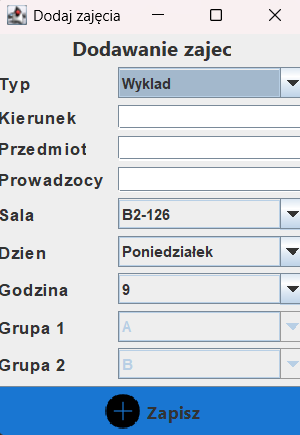
\includegraphics[width=0.45\textwidth]{figures/workApl/add_wyklad_panel.png}
\caption{Formularz dodawania zajęć typu Wykład}
\label{fig:add_wyklad}
\end{figure}

\clearpage

\section*{Formularz dodawania zajęć typu Laboratorium}

Na Rys. \ref{fig:add_lab} zaprezentowano formularz służący do dodawania zajęć typu \textbf{Laboratorium}. W tym przypadku możliwe jest przypisanie jednej grupy do zajęć – użytkownik wybiera ją w polu \texttt{Grupa 1}, natomiast \texttt{Grupa 2} pozostaje nieaktywne.

Formularz ten dostosowuje swoją funkcjonalność dynamicznie w zależności od wybranego typu zajęć. Przycisk \textbf{Zapisz} umożliwia dodanie danych po przejściu poprawnej walidacji.

\begin{figure}[H]
\centering
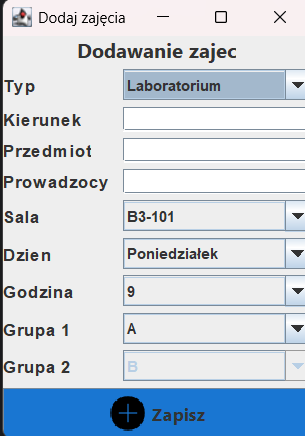
\includegraphics[width=0.45\textwidth]{figures/workApl/add_lab_panel.png}
\caption{Formularz dodawania zajęć typu Laboratorium}
\label{fig:add_lab}
\end{figure}

\clearpage

\section*{Formularz dodawania zajęć typu Projekt}

Jak przedstawiono na Rys. \ref{fig:add_projekt}, formularz ten umożliwia przypisanie dwóch grup do wspólnych zajęć typu \textbf{Projekt}. Dane te są zapisywane zarówno w tabeli \texttt{zajecia}, jak i w powiązanej tabeli \texttt{projekty}.

Użytkownik musi podać wszystkie wymagane informacje: kierunek, przedmiot, prowadzący, sala, dzień i godzina zajęć, oraz przypisać obie grupy projektowe. System weryfikuje poprawność danych oraz sprawdza potencjalne konflikty terminów przed zapisaniem rekordu.

\begin{figure}[H]
\centering
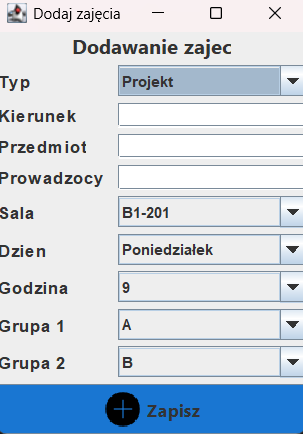
\includegraphics[width=0.45\textwidth]{figures/workApl/add_projekt_panel.png}
\caption{Formularz dodawania zajęć typu Projekt}
\label{fig:add_projekt}
\end{figure}

\clearpage

\section*{Formularz edycji zajęć}

Rys. \ref{fig:edit_panel} prezentuje panel edycji zajęć. Użytkownik może zaznaczyć rekord z tabeli głównego panelu i przejść do jego modyfikacji. Wszystkie dane z wybranego wiersza są automatycznie załadowane do formularza.

Po zakończeniu edycji wystarczy kliknąć przycisk \textbf{Zapisz}, aby zapisać zmiany w bazie danych. Formularz umożliwia edycję dowolnego typu zajęć — również typu \texttt{Projekt} i \texttt{Laboratorium}, przy czym zachowane są te same zasady walidacji co podczas dodawania.

\begin{figure}[H]
\centering
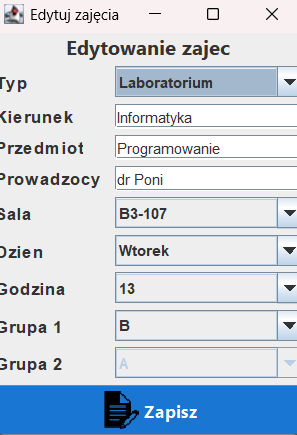
\includegraphics[width=0.45\textwidth]{figures/workApl/edit_panel.png}
\caption{Formularz edycji istniejących zajęć}
\label{fig:edit_panel}
\end{figure}
